
\section{FAQs}

\begin{enumerate}

\item \textbf{What to do in case of any communication or initialization failure while running examples?}
\newline Resetting or rebooting the board will help solving such issues.

\item \textbf{Why is there no output in my terminal application after cross-compiling and downloading an example on the MCU?}
\newline The code example on the MCU waits until the serial port of the board is opened. However, opening the port is not enough, the user has to ensure that also the DTR signal is set (this is required due to have higher compatibiliy among different terminal applications).


\item \textbf{How to fix libusb not found issue on macOS (arm64)?}

Please try the below steps to fix the issue.
\begin{enumerate}
    \item Install libusb:
    Libusb will be automatically installed as part of the COINES installation. However, If it’s not installed automatically, you can use Homebrew to install it. 
    \lstinline|brew install libusb|
    \newline After running above command, libusb should be installed on your system.
    \newline On Intel Mac: \path{/usr/local/lib}
    \newline On M1 Mac: \path{/opt/homebrew/lib}
    \item Add the path in \path{<installed_COINES_location>/coines.mk}
    \begin{figure}[H]
        \begin{center}
            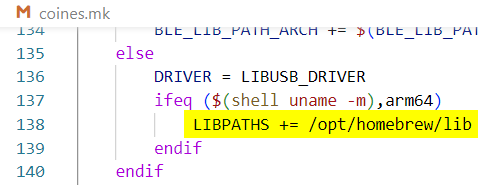
\includegraphics[width=0.6\textwidth]{coinesAPI_images/Mac_libusb_include.png}
            \caption{COINES file structure}
        \end{center}
    \end{figure}
\end{enumerate}

\item \textbf{How do I recover the original program when bootloader was erased accidentally on Application Board 3.x?}
\newline COINES SDK does not provide a way to restore the board to original state.

\item \textbf{How to run multiple application boards using COINES in a single computer?}
\newline When multiple USB devices are connected to a PC, by configuring Serial COM settings for a script, one can communicate with them separately. Please refer to \ref{serialComConfig} for implementation.

\end{enumerate}
For more FAQs, visit \href{https://community.bosch-sensortec.com/t5/MEMS-sensors-forum/bd-p/bst_community-mems-forum}{Bosch Sensortec MEMS sensors forum}.
